%This is a very basic  BE PROJECT PRELIMINARY template.

%############################################# 
%#########Author :  PROJECT###########
%#########COMPUTER ENGINEERING############


\documentclass[oneside,a4paper,12pt]{report}
%\usepackage{showframe}
%\hoffset = 8.9436619718309859154929577464789pt
%\voffset = 13.028169014084507042253521126761pt

\usepackage{graphicx}
\usepackage{fancyhdr}
\usepackage{pbox}
\fancypagestyle{plain}{%
  \fancyhf{}
  \fancyfoot[CE]{Maharashtra Institute of Technology, Department of Computer Engineering 2017-18}
  \fancyfoot[RE]{\thepage}
}
\pagestyle{fancy}
\fancyhead{}
\renewcommand{\headrulewidth}{0pt}
\footskip = 0.625in
\cfoot{}
\rfoot{}

\usepackage[]{hyperref}
\usepackage{tikz}
\usetikzlibrary{arrows,shapes,snakes,automata,backgrounds,petri}

\usepackage{tabularx}

\usepackage[nottoc,notlot,notlof,numbib]{tocbibind}
\usepackage[titletoc]{appendix}
\usepackage{titletoc}
\renewcommand{\appendixname}{Annexure}
\renewcommand{\bibname}{References}

\setcounter{secnumdepth}{5}

\usepackage{float}
\usepackage{subcaption}
\usepackage{multirow}

\usepackage[ruled,vlined]{algorithm2e}

\begin{document}
\setlength{\parindent}{0mm}
\begin{center}
{\bfseries SAVITRIBAI PHULE PUNE UNIVERSITY \\}
 \vspace*{1\baselineskip}
{\bfseries A  PROJECT REPORT ON \\}
 \vspace*{2\baselineskip}
{\bfseries \fontsize{16}{12} \selectfont Improving Human-Computer Interaction with Machine Emotion Intelligence using NAO Robot  \\ \vspace*{2\baselineskip}}
{\fontsize{12}{12} \selectfont SUBMITTED TOWARDS THE
 \\FULFILLMENT OF THE REQUIREMENTS OF \\

\vspace*{2\baselineskip}}
{\bfseries \fontsize{14}{12} \selectfont BACHELOR OF ENGINEERING (Computer
Engineering) \\
\vspace*{1\baselineskip}} 
{\bfseries \fontsize{14}{12} \selectfont BY \\ 
\vspace*{1\baselineskip}} 
\centering{Manas Kale         (B120024271) \\}
\centering{Rohit Patankar     (B120024292)  \\}
\centering{Saurabh Shirodkar  (B120024)  \\}
\centering{Shubham Punekar    (B120024304) \\}
\vspace*{2\baselineskip}
{\bfseries \fontsize{14}{12} \selectfont Under The Guidance of \\  
\vspace{\baselineskip}} 
Dr. V.Y. Kulkarni\\
%\includegraphics[width=100pt]{collegelogo.png} \\
\vspace{\baselineskip}
\begin{center}
	\textbf{Department of Computer Engineering}\\
	\bf{MAEER's MAHARASHTRA INSTITUTE OF TECHNOLOGY}\\
	\textbf{Kothrud, Pune 411 038}\\
	\textbf{2016-2017}
\end{center}

\end{center}

\newpage



\begin{figure}[ht]
\centering
%\includegraphics[width=100pt]{collegelogo.png}
\end{figure}


{\bfseries \fontsize{14}{12} \selectfont \centering{Maharashtra Institute of Technology, Pune}

\centering{DEPARTMENT OF COMPUTER ENGINEERING}
\vspace*{2\baselineskip}} 


\begin{center}
	\textbf{\underline{C E R T I F I C A T E}}\\
	\vspace{0.2in}
\end{center}

\centering{This is to certify that the Project Entitled}
\vspace*{.5\baselineskip} 


{\bfseries \fontsize{14}{12} \selectfont \centering{Improving Human-Computer Interaction with Machine Emotion Intelligence using NAO Robot}
\vspace*{0.5\baselineskip}}

\centering{Submitted by:}
{\bfseries \fontsize{14}{12} \selectfont \\ 
	\vspace*{1\baselineskip}} 
\centering{Manas Kale         (B120024271) \\}
\centering{Rohit Patankar     (B120024292)  \\}
\centering{Saurabh Shirodkar  (B120024)  \\}
\centering{Shubham Punekar    (B120024304) \\}
\vspace*{2\baselineskip}
\begin{quote}
is a bonafide work carried out by students under the supervision of Dr. V.Y. Kulkarni and it
is submitted towards the fulfillment of the requirement of Bachelor of Engineering (Computer Engineering).
\end{quote}
\noindent
\vspace{0.1 in}
\begin{quote}
	Prof. Dr. V.Y. Kulkarni\\
	(Internal Guide and Head of Computer Engineering Department)\\
	
	Place: Pune \hspace{2.2 in}  Date: 
\end{quote}

\newpage

\begin{center}
\textbf{PROJECT APPROVAL SHEET}
\end{center}
\begin{center}
Improving Human-Computer Interaction with Machine Emotion Intelligence using NAO Robot
\end{center}
\begin{center}
Is successfully completed by 
\end{center}
\begin{center}
Manas Kale         (B120024271) \\
Rohit Patankar     (B120024292)  \\
Saurabh Shirodkar  (B120024)  \\
Shubham Punekar    (B120024304) \\
\end{center}
\begin{center}
 at
 \end{center} 
 \begin{center}
 DEPARTMENT OF COMPUTER ENGINEERING
 \end{center}
 \begin{center}
 Maharashtra Institute of Technology, Pune
 \end{center}
 \begin{center}
 SAVITRIBAI PHULE PUNE UNIVERSITY,PUNE
 \end{center}
 
 \begin{center}
 ACADEMIC YEAR 2017-2018
 \end{center}
 \noindent
 \vspace{0,3 in}
 \begin{quote}
Dr. V.Y. Kulkarni (Dept. of Computer Engg.)
\end{quote}
\newpage

{  \newpage {\bfseries \fontsize{14}{12} \selectfont \centering{Acknowledgements} 
\vspace*{2\baselineskip}} \setlength{\parindent}{11mm} }
\begin{center}
	It gives us great pleasure in presenting the project report 
		on 
		{\bfseries \fontsize{12}{12} \selectfont 'Improving Human-Computer Interaction with Machine Emotion Intelligence using NAO Robot'}.
	\vspace*{1.5\baselineskip}
	
	We would like to take this opportunity to thank our internal guide and H.O.D.
		\textbf{Dr. V.Y. Kulkarni} for giving us all the help and guidance we needed. Her valuable suggestions were extremely helpful. We would also like to express our sincere appreciation to staff of department of Computer Engineering, Maharashtra Institute of Technology Pune, for their extended help and suggestions at every stage.\\
	In the end our special thanks to our college support staff for providing various resources such as  laboratory whenever we wanted with all needed software platforms, continuous internet connection, and air conditioning for our project work.
	\vspace*{1.5\baselineskip}
\end{center}

\begin{normalsize}

\tableofcontents
\listoffigures 
\listoftables

\begin{abstract}
In our project, we have focused on inculcating machine emotion intelligence using the NAO robot. Emotion detetion is a challenging problem partly because it is difficult to determine the features the might be reveleant to the task, and partly because the emotive states are overlapping and not mutually exclusive. Emotional state of a person at any given time is not categorical, but a value from a wide spectrum of emotions. Thus, we have pre-defined a limited set of emotions and focused on an ensemble approach by considering the interacting human's voice, spoken content as well as facial cues to detect the emotional state. We have used a pipeline of deep neural network for tone analysis, an SVM for facial feature analysis and a neural network for analysing the spoken text. By using a weighted function, an output is calculated from probability distributions for emotion labels predicted by all 3 modules. The robot will accept a multimodal input periodically and output the associated recognized emotion label on the user interface along with graphs to show the changing emotions with respect to every sample taken.
\end{abstract}


\chapter{Synopsis}

\section{Project Statement}
Improve Human Computer Interaction with Machine Emotional Intelligence using Nao Robot to: 
\begin{itemize}
\item recognize subjects based on their facial features and voice
\item analyse the facial features, speech text and the tone of speech to detect emotions
\item generate and emotive score based on a weighted scores from former analyses
\end{itemize}
\noindent
\vspace{0,2 in}

\section{Scope of the Problem}
\begin{itemize}
\item NAO robot will automatically and periodically analyze voice samples and facial cues in order to detect the emotional state of the person interacting with the robot.
\item Specified number of frames per second will be analysed for facial cues.
\item Audio segments will be analysed via tone for emotion detection.
\item Speech text extracted from the audio segments will be aggregated and analysed for emotion.
\item The robot will not be able to detect every single complex emotion, but will be limited to a subset of generalized emotions.

\end{itemize}

\newpage

\section{Goals and Objectives}
\begin{itemize}
	\item Knowing the emotional state of an individual can be crucial in determining what action is to be taken as a response.
	\item Recognizing the affective state of a human can be difficult for humans as well as computer systems. Many features can be considered such as voice samples, facial cues or even text written by the person to identify the emotional state of the individual.
	\item The major focus of the project is improving human-machine interaction using the NAO robot.
	\item The robot will accept the input from the person periodically in the form of speech samples, comprising of voice and text as well as facial cues and will interpret the current emotional state of the person.
	\item Although our main focus is on humanizing the NAO robot, there are myriad of other uses that can be achieved; some of which are:
	\begin{itemize}
		\item Development of an affect-aware city
		\item Add security layer at public venues to detect malicious intent and deal with hostage situation effectively
		\item Measure response and ratings in focus groups (consumer response to commercials etc)
		\item Wearables that help autistics discern emotion etc.
	\end{itemize}
\end{itemize}

\newpage
\section{Relevant mathematics associated with the Project}
\label{sec:math}
\begin{flushleft}
\textbf{System Description:}\\
The System is divided into three parts, each of which handles a mode of emotion recognition. Each part has it's own specification of inputs. However, the system as a whole has output in terms of final output emotion label as well as associated graphs. The system takes three types of inputs(audio, face and text samples) which are given to the associated part for emotion recognition.\\
\vspace{5mm}
Consider System as S:\\
S = \{ I, O, F, SC, FC \}\\
where,
\end{flushleft}
\begin{itemize}
	\item[--]I = Input
	\item[--]O = Output
	\item[--]F = Functions
	\item[--]SC = Success Cases
	\item[--]FC = Failure Cases
\end{itemize}
\vspace{5mm}
\begin{itemize}
\item \textbf{I}: Multimodal input captured using Camera and Microphone/ stored file\\
\vspace{3mm}
\textbf{I} = \{ Audio and Video sampling is customizable. However, the default sampling is at 1 second and in case of significant input, 5 second utteracnes are captured\}
\vspace{3mm}
\item \textbf{Output}: Distinct emotion label from the pre-defined set of emotions\\emotions = \{Neutral, Sadness/Fear, Frustration/Anger/Disgust, Happiness/Excitement/Surprise\}
\newpage
\item F : \{ F1, F2, F3\}\\
\vspace{2mm}
\begin{itemize}
	\item F1  =  \textbf{Data Preprocessing}\\
	\begin{itemize}
		\item \textbf{Audio Module}\\
		\begin{itemize}
			\item \textbf{Functions} =\newline  \{  \textbf{F1:} Determine threshold with amplitudes for silence \\ \begin{equation}
			threshold = \theta | \theta = max{S_0, .. ,S_k} \end{equation} where \(S_i\) = Sampled integer during base-line seconds used for measuring threshold\newline \\ \textbf{F2:} Generate MFCCs for each frame z(m)\\ \textbf{F3:} Generate MFCC matrix for segments. 2m+1 frames of 25 ms each are stacked to produce one segment x(m) of 265 ms each using slinding window of w = 10 ms \\ \begin{equation}
			x(m) = [z(m-w), ... z(m), ... z(m+w)]
			\end{equation} \newline\\ \textbf{F4:} Generate statistical features from probability distribution \\ \begin{equation}
			(f_1)^k = max_{S \epsilon U} P_s(E_k)
			\end{equation} where,\newline \(P_s(E_k)\) denotes the probability for kth emotion for segment S in the utterance U \}\newline
			
			
			\item \textbf{SC} = \{ Appropriate threshold selected for ambient noise, appropriate sliding window size selected to convert
			 audio frames into segments\}\newline
			 
			 
			\item \textbf{FC} = \{ Improper threshold for ambient noise resulting in no audio utterance being generated, improper window size selected resulting in improper MFCC matrix\} \\
		\end{itemize}
		\vspace{4mm}
		
		
		\item \textbf{Video Module}\\
		\begin{itemize}
			\item \textbf{Functions} = \{ \textbf{F1:}: Optimize contrast by performing histogram equilization \\ \textbf{F2:} Detect faces in the frame \\ \textbf{F3:} Map 68 landmarks onto the detected face \\ \textbf{F4:} Re-orient the face by taking the centroid of the detected landmarks and the normal \\ \textbf{F5:} Generate features by calculating distances and angles of the landmarks from the centroid and normal respectively \}\newline
			\item \textbf{SC} = \{ Faces detected in the frame, image having optimal contrast, only one face utilized from  multiple faces in the frame \}\newline
			\item \textbf{FC} = \{ Faces not detected in the frame, too dark/ bright/ blurred images for effective edge detection , face angle too oblique \}\newline
		\end{itemize}
		\vspace{4mm}
		\item \textbf{Speech Module}\\
			\begin{itemize}
			\item \textbf{Function} = \{ \textbf{transcribe()} : Takes the speech audio as input, and generates corresponding transcript.
			\textbf{transform()} - Transforms the transcript into a feature vector of a predefined format.
			\textbf{predict()} - Predicts the probabilities of the transcript belonging to each of the emotion labels. \}
			\newline
			\item \textbf{SC} = \{ Audio stream is clear enough to generate transcript properly, Stable internet connection available to access Google Speech to Text API,  Speech takes place in English language, Feature vector is not too sparse, and enough spoken words occur in the feature set to accurately discern between emotions \}
			\newline
			\item \textbf{FC} = \{ Too much noise in the audio stream to detect speech, Unstable internet connection preventing consistent access to Google Speech to Text API, Language other than English spoken, Feature vector generated is too sparse to accurately discern between emotions.  \}
			\newline
		\end{itemize}
	\end{itemize}
	\vspace{5mm}
	\item F2  =  \textbf{Training the Models}\\
	\begin{itemize}
		\item \textbf{Tone Module: }
		\begin{itemize}
			\item \textbf{Input} :
			\begin{enumerate}
				\item Prepocessed data in the form of MFCC matrix of segments composed from frames.
				\item  One feature vector contains 325 MFCCs (13 MFCCS for 25 frames each).				
			\end{enumerate}
		
			\item \textbf{Output} : Probability distribution for each segment \newline
			\item \textbf{Parameters} :
			\begin{enumerate}
				\item 3 hidden layers of 250 neurons each (250,250,250)
				\item Input layer contains 325 neurons as per the dimensionality of the feature vector
				\item Output layer is a softmax layer for probabilities of 4 emotion labels
				\item Activation function used is ReLU
				\item Learning algorithm is stochastic gradient descent
				\item Objective function is cross entropy error
			\end{enumerate}
		\end{itemize}
		\vspace{10mm}
		\item \textbf{Video Module: }
		\begin{itemize}
			\item \textbf{Input} :
			\begin{enumerate}
				\item A feature vector of 136 dimensions (68 landmarks and 68 angles)
			\end{enumerate}
		
			\item \textbf{Output} :
			\begin{enumerate}
			\item Probability distribution of the 6 emotion labels
			\end{enumerate}
	
			\item \textbf{Parameters} :
			\begin{enumerate}
			\item SVM with a linear kernel is used 
			\end{enumerate} 
		\end{itemize}
		\vspace{10mm}
		\item \textbf{Speech Module: }
	\begin{itemize}
		\item \textbf{Input} 
		\begin{enumerate}
			\item 
			\item
			\item
			\item
			\item
		\end{enumerate}
		
		\item \textbf{Output} = \{ 
		\begin{enumerate}
			\item 
			\item
			\item
			\item
			\item
		\end{enumerate}  \}
		
		\item \textbf{Parameters} = \{ 
		\begin{enumerate}
			\item 
			\item
			\item
			\item
			\item
		\end{enumerate}  \}
		
		\}
	\end{itemize}
	\end{itemize}
		
\vspace{4mm}
	\item \textbf{F3 = Emotion Recognition}\\
	\begin{itemize}
		\item \textbf{Input: } Probability distributions for all emotion labels predicted by individual classifiers ( \( P_c(k) \) ) ; c = 1,2,3 for video, tone and speech modules respectively.
		\newline
		\item \textbf{Output: } Weighted probability distribution for emotion labels from stacked classifiers
		\newline
		\item \textbf{Processing: } Weighted average of probabilities from classifiers which are weighted by a time decaying factor
		\begin{equation}
		P_{(k)} = \sum_{c=1}^{3} P_c(k) w_c
		\end{equation}
		where,\newline \(w_c\) = w\( - \Delta\)w ;\newline \(\Delta w = d * t\) ; \newline d = decay factor ; \newline w = default maximum weight
	\end{itemize}
\end{itemize}
\end{itemize}
\newpage


\chapter{Technical Keywords}

\section{Area of Project}
\begin{center}
	The area of our project lies in the intersection of three distinct areas which are Machine Learning, Computer Vision and Natural Language Processing.
\end{center}

\section{Technical Keywords}

 \begin{itemize}
   \item 	\textbf{Machine Learning: } Machine learning is a field of computer science that uses statistical techniques to give computer systems the ability to "learn" with data, without being explicitly programmed.
 \item \textbf{Computer Vision: } Computer vision is an interdisciplinary field that deals with how computers can be made to gain a high-level understanding from digital images or videos.
 \item	\textbf{Affective Computing: } Affective computing is the study and development of systems and devices that can recognize, interpret, process, and simulate human affects. It is an interdisciplinary field spanning computer science, psychology, and cognitive science.
 \item \textbf{Neural Network: } Artificial neural networks or connectionist systems are computing systems vaguely inspired by the biological neural networks that constitute animal brains.
 
 \item \textbf{Deep Neural Network: } Deep Neural Network (DNN) is an artificial neural network (ANN) with multiple hidden layers between the input and output layers.[9][2] DNNs can model complex non-linear relationships.
 
 
 \item \textbf{SVM: } In machine learning, support vector machines are supervised learning models with associated learning algorithms that analyze data used for classification and regression analysis.
 
 \end{itemize}

\chapter{Introduction}
\section{Project Idea}
 The basic idea behind our project was to combine the various forms of input that one usually analyses in order to determine a person's emotional state.

\vspace{\baselineskip}
\section{Motivation of the Project}  
\begin{itemize}
	
\item Majority of work done towards emotion detection is focused on a single mode i.e. audio/ video/ text. There is limited practical work done be considering multimodal inputs.

\item In general literature available today, numerous features have been developed , however performance of classifiers is still limited as the emotional states cannot be accurately distinguished by a well-defined set of discriminating features.

\item By considering multimodal input, the final output is completely influenced by the quality and accuracy of the input itself, thus in scenarios where one mode of input becomes unreliable, the output can be provided by another mode thereby maintaining the accuracy of identification of emotions.

\end{itemize}

\newpage

\section{Literature Survey}
\begin{itemize}
	\item \textbf{Jeong-Sik Park,  Gil-Jin Jang:  "Implementation of Voice emotion Recognition for Interaction with Mobile Agent , ACM 2014"} \cite{park15_implem_voice_emotion_recog_inter} \\
	The paper proposes a simple smartphone interface framework which consists of detection of human voice, extraction of emotional features and identification of an emotional state. Energy based approach for detection of human voice is selected in which if continues estimates of spectral energy of consecutive frames exceeds a pre-determined threshold, the region is regarded as starting point of voice signal. The pitch, log-energy, and Mel-Frequency Cepstral Coefficient (MFCC) are selected for extraction of emotional features which make a feature vector sequence. Acoustic features vectors extracted are analyzed and compared with patterns for each emotion type. Guassian Mixture Model is the classification algorithm used. This approach achieved 70.1\% correctness within 1s response time. The future work suggested is applying proposed concepts for human-machine interaction in personal agent applications.
	
		\vspace{5mm}
	\item \textbf{ Yu Gu, Eric Postma, Hai-Xing Lin:  "Vocal Emotion Recognition using Log-Gabor Filters , ACM 2015"} \cite{gu15_vocal_emotion_recog_log_gabor_filter} \\
	The propsed work utilizes 2d Gabor filters in order to decompose the associated spectogram in order to perform a spectro-temporal analysis of affective vocalizations. Instead of including all potentially relevant features which leads of dimensionality problem and subsequent degradation of performance, the work uses feature learning in which relevant features are automatically obtained from raw speech signals. However this leads to considerable computational resouces. Hence, no. of features is kept to minimum. By performing analysis on local specto-temporal structure, the spectrogram is treated as an image and standard image processing is implemented. Comparative evaluation of MFCC and LPCC features, untuned and tuned Gabor filters and all above combinations is done. SVM is used as a classifier. The confusion matrix for performance using tuned Gabor Filters provide a maximum of 91.6\% accuracy whereas a combination of acoustic features and Gabor filter provides 93.5% accuracy.
		\vspace{5mm}
	 \item \textbf{Gloria Zen, Elisa Ricci, Nicu Sebe:  "Unsupervised Domain Adaption for Personalized Facial Emotion Recognition, ACM 2014"} \cite{zen14_unsup_domain_adapt_person_facial_emotion_recog} \\
	A personalization approach is proposed in which only unlabeled target-specific data are required. A new method to represent the source sample distribution based on only Support Vectors of source classifiers is proposed. Regression framework is used to learn a mapping between a marginal distribution of the data points associated to a given person and the parameters of his/her personalized classifier which is represented by a set of Support Vectors of linear classifier in the source case and by all unlabeled data points in the target case.
	
		\vspace{5mm}
	\item \textbf{Ahmed Mustafa Mahmoud,  Wan Haslina Hassan:  "Determinism in Speech Pitch Relation to Emotions, ICIS 2009"} \cite{mahmoud09_deter} \\
	A deterministic rule-based text-to-speech emotional synthesis approach is proposed to generate emotional speech using semitonic interval-driven rules. Emotional speech samples are analyzed and intervals are extracted using praat tool. Objective evaluation compares sysnthesized voice to natural voice and calculates difference as an error function by considering mean square error as a measure of similarity. New emotional states may be defined using same proposed approach. Algorithms that integrate two or more emotional states may be combined to generate a variety of complex emotions.
		\vspace{5mm}
	\item \textbf{Nancy Semwal,  Abhijeet Kumar, Sakthivel Narayanan:  "Automatic Speech Emotion Detection using Multi-Domain Acoustic Feature Selection and Classification,  IEEE 2015"} \cite{semwal17_autom} \\
	The proposed approach concentrated on determining emotions from speech signals. Various acoustic features such as energy, zero-crossing rate(ZCR), fundamental frequency, Mel Frequency Cepstral Coefficient are extractedfor short term, overlapping frames derived from the input signal. A feature vector for every utterance is then constructed by analyzing mean, median, etc. over all frames. Sequential Backward Selection is used with K-fold cross validation to select a subset of useful features. Detection of emotions is done by classifying respective features from the full candidate feature vectors into classes, using either a pre-trained SVM or a Linear Discriminant Analysis classifier. Accuracy of 80\% was obtained when tested on EmoDB dataset.
		\vspace{5mm}
	\item \textbf{Lei Pang,  Chong-Wah Ngo:  "Multimodal Learning with Deep Boltzmann Machine for Emotion Prediction,  ACM 2015"} \cite{pang15_mutlim_learn_deep_boltz_machin} \\
	In contrast to existing works which concentrate on either Audio, text or video, a joint density model is proposed over the space of multi-modal inputswith Deep Boltzmann Machine. The model is trained directly on user-generated Web videos without any labelling effort. Multiple layers of hidden units and multiple modalities make learning difficult, hence learning is split into 2 stages. First, each RBM component is pre trained using greedy layerwise strategy. Then, learnt parameters are used to initialize the parameters of all layers in DBM and then the multimodal DBM is trained to finetune different modalities in a unified way. A major factor is that the deep architecture enlightens the possibility of discovering highly non-linear relationships between low-level features across different modalities. A performance improvement of 7.7\% in classification accuracy is observed.
	
		\vspace{5mm}
	\item \textbf{Benjamin Guthier,  Rajwa Alharthi,  Rana Abaalkhail,  Abdulmotaleb El Saddik:  "Detection and Visualization of Emotions in an Affect-Aware City,  ACM"} \cite{guthier14_detec_visual_emotion_affec_aware_city} \\
	In the proposed work, emotions are represented as four-dimensional vectors of pleasantness, arousal, dominance and unpredictability. In the training phase, emotion word hashtags in the messages are used as the ground-truth emotion contained in a message. A neural network is trained by using the presence of words, hashtags and emoticons in the message as features. During the live phase, these features are extracted from geo-tagged Twitter messages and given as input to neural-network. The detected emotions are aggregated over space and time and visualized on a map of the city.
		\vspace{5mm}
	\item \textbf{Huaizu Jiang, Erik Learned-Miller:  "Face Detection with Faster R-CNN"} \cite{jiang17_face_detec_faster_r_cnn} \\
	Most approaches to face detection are still based on the R-CNN framework , leading to limited accuracy and processing speed. In this paper, investigations regarding the application of Faster R- CNN  which has demonstrated impressive results on various object detection benchmarks, to face detection have been made. By training a Faster R-CNN model on the large scale WIDER face dataset, state-of-the-art results on the WIDER test set as well as two other widely used face detection benchmarks, FDDB and the recently released IJB-A have been presented.
		\vspace{5mm}
	
	\item \textbf{Wei Jang, Wei Wang:  "Face Detection and Recognition for Home Service Robots wth End-To-End Deep Neural Networks, IEEE 2017"} \cite{jiang17_face} \\
	This paper proposes an effective end-to-end face detection and recognition framework based on deep convolutional neural networks for home service robots. State-of-the-art region proposal based deep detection network has been combined with he deep face embedding network into an end-to-end system, so that the detection and recognition networks can share the same deep convolutional layers, enabling significant reduction of computation through sharing convolutional features. The detection network is robust to large occlusion, and scale, pose, and lighting variations. The recognition network does  not require explicit face alignment, which enables an effective training strategy to generate a unified network. A practical robot system is also developed based on the proposed framework, where the system automatically asks for a minimum level of human supervision when needed, and no complicated region-level face annotation is required. Experiments are conducted over WIDER and LFW benchmarks, as well as a personalized dataset collected from an office setting, which demonstrate state-of-the-art performance of the system.
		\vspace{5mm}
	\item \textbf{Rajesh K M, Naveenkumar M:  "A Robust Method for face Recognition and Face Emotion Detection System using Support Vector Machines,  IEEE 2016"} \cite{rajesh16} \\
	This paper presents framework for real time face recognition and face emotion detection system based on facial features and their actions. The key elements of Face are considered for prediction of face emotions and the user. The variations in each facial feature are used to determine the different emotions of face. Machine learning algorithms are used for recognition and classification of different classes of face emotions by training of different set of images. In this context, by implementing herein algorithms would contribute in several areas of identification, psychological researches and many real world problems. The proposed algorithm is implemented using open source computer vision (OpenCV) and Machine learning with python.
	
		\vspace{5mm}
	\item \textbf{Jie Shen, Ognjen Rudovic, Shiyang Cheng, Maja Pantic:  "Sentiment Apprehension in Human-Robot Interaction with NAO"} \cite{shen15_sentim_nao} \\
	In this paper, the influence of sentiment apprehension by robots (i.e., robots ability to reason about the users attitudes such as judgment / liking) on the user engagement has been studied. Two versions of mimicry game are studied: in the first, NAO was solely mimicking facial expressions of the users, while in the second he was also providing a feedback based on the sentiment apprehension. A total of 32 participants (7 female, 25 male) were recruited for this experiment, and the results show that the participants in the second group spent more time interacting with the robot and played more rounds of the mimicry game. After experiencing both versions of the game, ratings given by the participants indicate (with 99\% confidence) that the game with sentiment apprehension is more engaging than the baseline version.
		\vspace{5mm}
	
	\item \textbf{Dario Bertero, Pascale Fung:  "A First Look into Convolutional Neural Network for Speech Emotion Detection,  IEEE 2017"} \cite{bertero17_convol_neural_networ} \\
	A real-time Convolutional Neural Network model for speech emotion detection. Our model is trained from raw audio on a small dataset of TED talks speech data, manually annotated into three emotion classes: Angry, Happy and Sad. It achieves an average accuracy of 66.1\%, 5\% higher than a feature-based SVM baseline, with an evaluation time of few hundred milliseconds. An in-depth model visualization and analysis is also provided.  How the neural network effectively activates during the speech sections of the waveform regardless of the emotion, ignoring the silence parts which do not contain information has also been shown. On the frequency domain the CNN filters distribute throughout all the spectrum range, with higher concentration around the average pitch range related to that emotion. Each filter also activates at multiple frequency intervals, presumably due to the additional contribution of amplitude-related feature learning.n
		\vspace{5mm}
	\item \textbf{Kun Han, Dong Yu, Ivan Tashev:  "Speech Emotion Recognition and Extreme Learning Machine, INTERSPEECH 2014"} \cite{han14_speec_emotion_recog_using_deep} \\
	Speech emotion recognition is a challenging problem partly because it is unclear what features are effective for the task. In this paper an approach is proposed to utilize deep neural networks (DNNs) to extract high level features from raw data and it is shown that they are effective for speech emotion recognition. First an emotion state probability distribution is produced for each speech segment using DNNs. Then utterance-level features from segment-level probability distributions are constructed. These utterancelevel features are then fed into an extreme learning machine (ELM), a special simple and efficient single-hidden-layer neural network, to identify utterance-level emotions. The experimental results demonstrate  that the proposed approach effectively learns emotional information from low-level features and leads to 20\% relative accuracy improvement compared to the state-of-the-art approaches.
	
		\vspace{5mm}
	\item \textbf{Dan Duncan, Gautam Shine, Chris English:  "Facial Emotion Recognition in Real Time"} \cite{duncan16_facial_emotion_recog_real_time} \\
	This paper proposes a convolutional neural network for classifying human emotions from dynamic facial expressions in real time. Transfer learning is used on the fully connected layers of an existing convolutional neural network which was pretrained for human emotion classification. A variety of datasets and homebrewed dataset is used to train the model. Overall training accuracy of 90.7\% and test accuracy of 57.1\% is achieved. A live video stream connected to a face detector feeds images to neural network. The network subsequently classifies an arbitrary number of faces per image simultaneously in real time. This paper essentially demonstrates the feasibility of implementing neural networks in real time to detect human emotions.
	
		\vspace{5mm}
	\item \textbf{Lifeng Shang, Zhengdong Lu, Hang Li:  "Neural Responding Machine for Short-Text Conversation"} \cite{shang15_neural_respon_machin_short_text_conver} \\
	This paper proposes Neural Responding Machine (NRM), a neural network-based response generator for Short-Text Conversation. NRM takes the general encoderdecoder framework: it formalizes the generation of response as a decoding process based on the latent representation of the input text, while both encoding and decoding are realized with recurrent neural networks (RNN). The NRM is trained with a large amount of one-round conversation data collected from a microblogging service. Empirical study shows that NRM can generate grammatically correct and content-wise appropriate responses to over 75\% of the input text, outperforming stateof- the-arts in the same setting, including retrieval-based and SMT-based models(Statistical Machine Translation or a generative model).
	\vspace{5mm}
	
	\item \textbf{Joost Broekens:  "Emotion and Reinforcement: Affective Facial Expressions Facilitate Robot Learning"} \cite{broekens07_emotion} \\
	Computer models can be used to investigate the role of emotion in learning. Here weThis paper presents EARL framework for the systematic study of the relation between emotion, adaptation and reinforcement learning (RL). EARL enables the study of communicated affect as reinforcement to the robot. In humans, emotions are crucial to learning. For example, a parent observing a child uses emotional  expression to encourage or discourage specific behaviors. Emotional expression can therefore be a reinforcement signal to a child. We hypothesize that affective facial expressions facilitate robot learning, and compare a social setting with a non-social one to test this. The non-social setting consists of a simulated robot that learns to solve a typical RL task in a continuous grid-world environment. The social setting additionally consists of a human (parent) observing the simulated robot (child). The humans emotional expressions are analyzed in real time and converted to an additional reinforcement signal used by the robot; positive expressions result in reward, negative expressions in punishment. It is quantitatively shown that the social robot indeed learns to solve its task significantly faster than its “non-social sibling. This paper concludes that this presents strong  evidence for the potential benefit of affective communication with humans in the reinforcement learning loop.
	
\end{itemize}


\chapter{Problem Definition and scope}
\flushleft
\section{Problem Statement}
\begin{itemize}
\item Our project addresses the lack of a system in practice today which considers more than one method of emotion recognition at the same time. Our goal is to design a system that considers audio, facial cues as well as the content spoken to recognize the emotion the speaker is experiencing. Making the system work in near-real time is also crucial to address the effectiveness of emotion recognition in a real-life scenario.\\
\end{itemize}
\vspace{5mm}

 \section{Statement of scope}
	\begin{itemize}  
	\item	A description of the software with Size of input, bounds on input, input validation, input dependency, i/o state diagram, Major inputs, and outputs are described without regard to implementation detail.
	\item The scope identifies what the product is and is not, what it will and won’t do, what it will and wont contain.
	
	
	\item The system will accept three inputs. Out of the three inputs, two will be directly picked up by the camera and microphone on the robot.
	\item The third input will be given to the system after undergoing a Speech-to-Text conversion.
	\item The audio input will be approximately 5 seconds long in .wav format.
	\item The video frames will be captured every second.
	\item After outputs are displayed, the files will be deleted to address the storage space requirement.
	\item The system will give the output in the form of an emotion label after successful emotion recognition.
	\item However, this label will be from a pre-defined set of emotions.
	\item For successful Speech-to-Text conversion, steady internet connection is required.
	\item The system will simply display a string representing the emotion and not generate any response to address that emotion.
	\item The output will also contain graphs which will indicate the how the emotional state of a person has changed over time.
	\end{itemize}

\vspace{4mm}
\section{Major Constraints}
\begin{itemize}
\item Any constraints that will impact the manner in which the software is to be specified, designed, implemented or tested are noted here.
\item The sensors on the NAO robot must be fully operational
\item Necessary python environment should be set up (preferably Anaconda)
\item Necessary python packages installed (pip, numpy, sklearn)

\end{itemize}
\vspace{4mm}
\section{Methodologies of Problem solving and efficiency issues}
\begin{itemize}
	\item The single problem can be solved by different solutions.  This considers the performance parameters for each approach. Thus considers the efficiency issues.
\end{itemize}
\vspace{4mm}
\section{Outcome}
\begin{itemize}
\item Effective emotion recognition in the form periodic emotion labels displayed.
\item Emotion recognition accuracy maintained by dynamically considering different inputs when one mode becomes unavailable.

\end{itemize}
\vspace{4mm}
\section{Applications}
\begin{itemize}
\item Development of an affect-aware city
\item Add security layer at public venues to detect malicious intent and deal with hostage situation effectively
\item Measure response and ratings in focus groups (consumer response to commercials etc)
\item Wearables that help autistics discern emotion etc.
\end{itemize}
\vspace{4mm}
\section{Software Resources Required}
\begin{enumerate}
	\item Operating System: Linux 64-bit
	\item IDE: Anaconda (Conda), Microsoft Visual Studio Code
	\item Programming Language: Python 3.6
	\item Libraries: numpy, sklearn, OpenCV, dlib, pyAudio, google-api-python-client
	\item Framework for UI: Flask, Bootstrap HTML Framework, any web browser
	\item Google Cloud API: account, key
\end{enumerate}
\vspace{10mm}
\section{Hardware Resources Required}

\begin{table}[!htbp]
	\begin{center}
		\def\arraystretch{3}
		\begin{tabular}{| c | c | c | m{3cm} |}
			\hline
			Sr.No. & Parameter & Minimum Requirement	& Justification \\ \hline
			1 &	CPU Speed &	 3 GHz  & Ensures that modules are trained in a timely manner\\ \hline
			2 &	GPU  &	4 GB+RAM &  Ensures that modules are trained in a timely manner\\ \hline
			3 & RAM & 8GB & To process large amount of training data\\ \hline
			4 & NAO Robot Camera+Mic & 320x240, 16000Hz & Getting accurate input \\ \hline
		\end{tabular}
	\end{center}
	\caption{Hardware Requirments}
	\label{tab:hw_req}
\end{table}


\chapter{Project Plan}

\section{Project Estimates}
                 Use Waterfall model and associated streams derived from assignments 1,2, 3, 4 and 5( Annex A and B) for estimation. 
\subsection{Reconciled Estimates}
\subsubsection{Cost Estimate}

\subsubsection{Time Estimates}


\subsection{Project Resources}
         \begin{itemize}
         \item Required hardware resources for training classifiers are available.
         \item Licensed softwares and libraries are available.
         \item Datasets and libraries used are provided under licenses which allow free use for non-commercial purposes. 
         \item The training of deep neural networks largely constitues the time requirements for the projects involving deep learning.
         \item Datasets and libraries are provided with licenses which allow use for non-commercial purposes.
         \item GNU GPL license, MIT license and Apache license allow use of datasets and libraries for non-commercial purposes. GNU GPL allows free use and  distribution of software under its license, as long as it's derivatives follow the same licensing model.
        \end{itemize}
         

\section{Risk Management w.r.t. NP Hard analysis}

\subsection{Risk Identification}
The possible risks are identified by considering the SRS, high-level and low-level design strategy. The risks are considered by evaluating the risk scenarios against various design, development and testing conditions. Each risk is categorized as per the categories mentioned in \cite{bookPressman}. Please refer table \ref{tab:risk} for all the risks.
\vspace{10mm}
\begin{table}[!htbp]
	\begin{center}
		%\def\arraystretch{1.5}
		\def\arraystretch{1.5}
		\begin{tabularx}{\textwidth}{| c | X | c | c | c | c |}
			\hline
			\multirow{2}{*}{ID} & \multirow{2}{*}{Risk Description}	& \multirow{2}{*}{Probability} & \multicolumn{3}{|c|}{Impact} \\ \cline{4-6}
			& & &	Schedule	& Quality	& Overall \\ \hline
			1	& Inconsistent datasets	& Low	& High	& High	& High \\ \hline
			2	& Skewed training data	& Low	& Low	& Low	& Low \\ \hline
			3	& All three inputs noisy at once	& Medium	& Medium	& Very High	& High \\ \hline
			4	& NAO interface restrictions	& Low	& Low	& High	& High \\ \hline
		\end{tabularx}
	\end{center}
	\caption{Risk Table}
	\label{tab:risk}
\end{table}


\begin{table}[!htbp]
	\begin{center}
		%\def\arraystretch{1.5}
		\def\arraystretch{1.5}
		\begin{tabular}{| c | c | c |}
			\hline
			Probability & Value &	Description \\ \hline
			High &	Probability of occurrence is &  $ > 75 \% $ \\ \hline
			Medium &	Probability of occurrence is  & $26-75 \% $ \\ \hline
			Low	& Probability of occurrence is & $ < 25 \% $ \\ \hline
		\end{tabular}
	\end{center}
	\caption{Risk Probability definitions}
	\label{tab:riskdef}
\end{table}

\begin{table}[!htbp]
	\begin{center}
		%\def\arraystretch{1.5}
		\def\arraystretch{1.5}
		\begin{tabularx}{\textwidth}{| c | c | X |}
			\hline
			Impact & Value	& Description \\ \hline
			Very high &	$> 10 \%$ & Schedule impact or Unacceptable quality \\ \hline
			High &	$5-10 \%$ & Schedule impact or Some parts of the project have low quality \\ \hline
			Medium	& $ < 5 \% $ & Schedule impact or Barely noticeable degradation in quality Low	Impact on schedule or Quality can be incorporated \\ \hline
		\end{tabularx}
	\end{center}
	\caption{Risk Impact definitions}
	\label{tab:riskImpactDef}
\end{table}

\vspace{10mm}
\subsection{Overview of Risk Mitigation, Monitoring, Management}

Following are the details for each risk.
\begin{table}[!htbp]
	\begin{center}
		%\def\arraystretch{1.5}
		\def\arraystretch{1.5}
		\begin{tabularx}{\textwidth}{| l | X |}
			\hline 
			Risk ID	& 1 \\ \hline
			Risk Description	& Inconsistent Datasets \\ \hline
			Category	& Development Environment. \\ \hline
			Source	&  Improper desciption and samples on the website\\ \hline
			Probability	& Low \\ \hline
			Impact	& High \\ \hline
			Response	& Data cleaning by validating audio/video files against file name \\ \hline
			Strategy	& Data preprocessing \\ \hline
			Risk Status	& Occurred and mitigated \\ \hline
		\end{tabularx}
	\end{center}
	\label{tab:risk1}
\end{table}

\begin{table}[!htbp]
	\begin{center}
		%\def\arraystretch{1.5}
		\def\arraystretch{1.5}
		\begin{tabularx}{\textwidth}{| l | X |}
			\hline 
			Risk ID	& 2 \\ \hline
			Risk Description	& Skewed Training Data \\ \hline
			Category	& Development Environment \\ \hline
			Source	& Diversity in dataset absent \\ \hline
			Probability	& Low \\ \hline
			Impact	& High \\ \hline
			Response	& Droping the dataset in favour of a more comprehensive one \\ \hline
			Strategy	& Validating as much of the dataset as possible  \\ \hline
			Risk Status	& Identified\\ \hline
		\end{tabularx}
	\end{center}
	\label{tab:risk2}
\end{table}

\begin{table}[!htbp]
	\begin{center}
		%\def\arraystretch{1.5}
		\def\arraystretch{1.5}
		\begin{tabularx}{\textwidth}{| l | X |}
			\hline 
			Risk ID	& 3 \\ \hline
			Risk Description	& All inputs noisy at once \\ \hline
			Category	& Development Environment \\ \hline
			Source	& Software Design Specification documentation review. \\ \hline
			Probability	& Medium \\ \hline
			Impact	& High \\ \hline
			Response	& Skip the accepted inputs until one input becomes accurate to ensure real-time response \\ \hline
			Strategy	& Dynamically switching between inputs and displaying previously identified emotion \\ \hline
			Risk Status	& Identified and Mitigated \\ \hline
		\end{tabularx}
	\end{center}
	\label{tab:risk3}
\end{table}

\begin{table}[!htbp]
	\begin{center}
		%\def\arraystretch{1.5}
		\def\arraystretch{1.5}
		\begin{tabularx}{\textwidth}{| l | X |}
			\hline 
			Risk ID	& 3 \\ \hline
			Risk Description	& Description 3 \\ \hline
			Category	& Technology \\ \hline
			Source	& This was identified during early development and testing. \\ \hline
			Probability	& Low \\ \hline
			Impact	& Very High \\ \hline
			Response	& Accept \\ \hline
			Strategy	& Example Running Service Registry behind proxy balancer  \\ \hline
			Risk Status	& Identified \\ \hline
		\end{tabularx}
	\end{center}
	\label{tab:risk3}
\end{table}

\section{Project Schedule}  
\subsection{Project task set}  
Major Tasks in the Project stages are:
\begin{itemize}
  \item Task 1:
  \item Task 2: 
  \item Task 3: 
  \item Task 4: 
  \item Task 5: 
\end{itemize}

\subsection{Task network}  
Project tasks and their dependencies are noted in this diagrammatic form.
\subsection{Timeline Chart}  
A project timeline chart is presented. This may include a time line for the entire project.
Above points should be covered  in Project Planner as Annex C and you can mention here Please refer Annex C for the planner

 
\section{Team Organization}
The manner in which staff is organized and the mechanisms for reporting are noted.  
\subsection{Team structure}
The team structure for the project is identified. Roles are defined.

\subsection{Management reporting and communication}
Mechanisms for progress reporting and inter/intra team communication are identified as per assessment sheet and lab time table.
 
\chapter{Software requirement specification  }

\section{Introduction}
\subsection{Purpose and Scope of Document}
\hspace{15mm}The purpose of the Software Requirements Specification document is to build a system to effectively recognize emotions at real-time to develop an emotionally aware robot as well as provide help to autistic people. The approach used for this task is a novel way of considering three input modules instead of just one. The different inputs used are the video frames, audio samples and the speech text. This document aims to identify the different and distinct design elements of the project as well as articulate the various requirements needed to make this project successful. The scope is limited to recognizing the emotions and not responding or generating any context related response. Also, the emotions considered for recognizing are limited to a pre-defined mutually-exlusive set of {Happiness, Anger, Neutral, Sadness}. The UML standard is adopted to represent the various diagrams which include Use-Case Diagram, Activity Diagram, Class Diagram, Sequence Diagram, State Diagram.
\newpage
\subsection{Intended Audience and Reading Suggestion}
\hspace{15mm}This project is a prototype for an emotion recognition system and it is restricted within the college premises. The project has been implemented for research purposes under the guidance of the Computer Department H.O.D Dr. V.Y. Kulkarni. This project is useful for individuals looking for a way to perform emotion recognition to use it a targeted application as well as a way to process multimodal inputs simultaneously.
\section{Usage Scenario}
This section provides various usage scenarios for the system to be developed.
\subsection{Use-cases}
All possible use-cases for the system are presented in the following table:
\begin{table}[!htbp]
\begin{center}
%\def\arraystretch{1.5}
\def\arraystretch{1.5}
\begin{tabularx}{\textwidth}{| c | X | X | X | X |}
\hline
Sr No.	& Use Case	& Description	& Actors	& Assumptions \\
\hline
1 & Take audio,video samples & Audio is captured whenever there is a 5 sec continuous utterance, Video is captured when a face is detected & Camera, Mic(Modelling actors) & Camera, Mic is initialized \\
\hline
2 & Emotion Recog using Video Module & Emotion is recognized by analyzing the orientation of the facial landmarks & Server & Face is detected\\
\hline
3 & Emotion Recog using Audio Module & Enabled when energy of sample is above a threshold, analyzed using energy \& MFCCs & Server & Audio energy above threshold\\
\hline
4 & Emotion Recog using Text Module & Speech-to-text conversion is done, feeding transcript as feature vector to classifier & Server & The transcript does not contain out-of-place words.\\
\hline
5 & Display emotion label & Final recognized emotion is displayed on the web interface & Web interface, Server & Appropriate weights are assigned previously\\
\hline
6 & Perform Speech-To-Text & Converts audio sample into transcripts & Google API, Server & Internet connection available\\
\hline 
\end{tabularx}
\end{center}
\caption{Use Cases}
\label{tab:usecase}
\end{table}
\newpage
\subsection{Use Case View}
The following gives the Use Case Diagram for the proposed system.
\begin{center}
	\begin{figure}[!htbp]
		\centering
		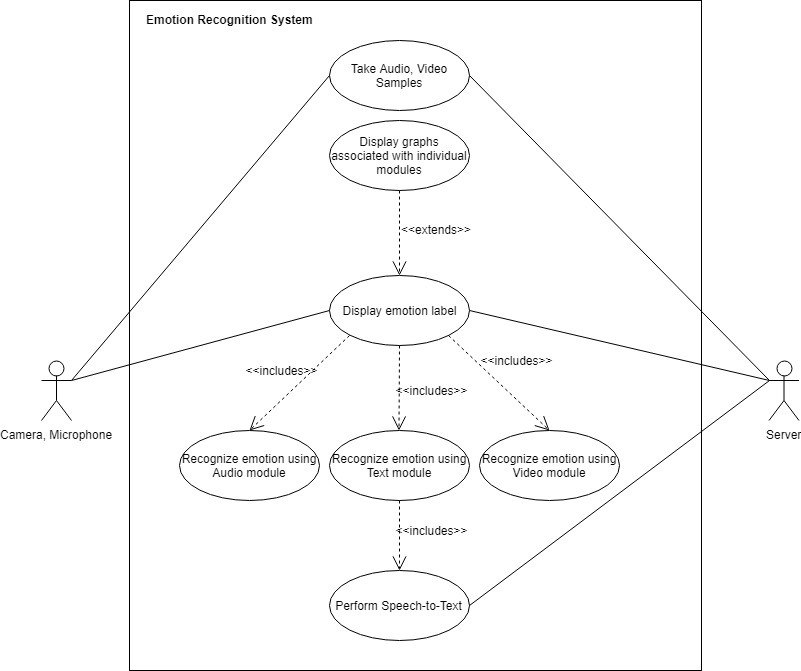
\includegraphics[width=\textwidth]{use_case_proj.jpg}
	  \caption{Use case diagram}
	  \label{fig:usecase}
	\end{figure}
\end{center}  
\newpage


\section{Functional Model and Description}
\hspace{15mm}Inputs in the form of audio samples and video frames from a human through a camera and microhpone. The System works on 3 distinct classifiers, each trained to handle a particular form of input. The audio input is given to the "Audio Recorder" whereas the video frames are given to the Video module. The Audio Recorder further sends the input to the Tone Analysis module and the Text Module. Each module runs their respective algorithm to recognize the emotions and assign their emotion label. The three labels are then sent to the web interface and the combined output is sent to the main process.
\subsection{Data Flow Diagram}   
\begin{center}
	\begin{figure}[!htbp]
		\centering
		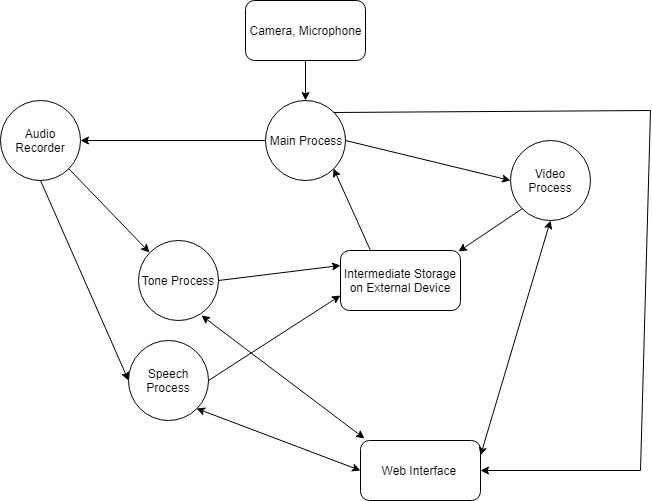
\includegraphics[width=\textwidth]{dataflow_proj.jpg}
		\caption{Dataflow diagram}
		\label{fig:dataflowdiag}
	\end{figure}
\end{center}  
\newpage

\subsection{Class Diagram}
\begin{center}
	\begin{figure}[!htbp]
		\centering
		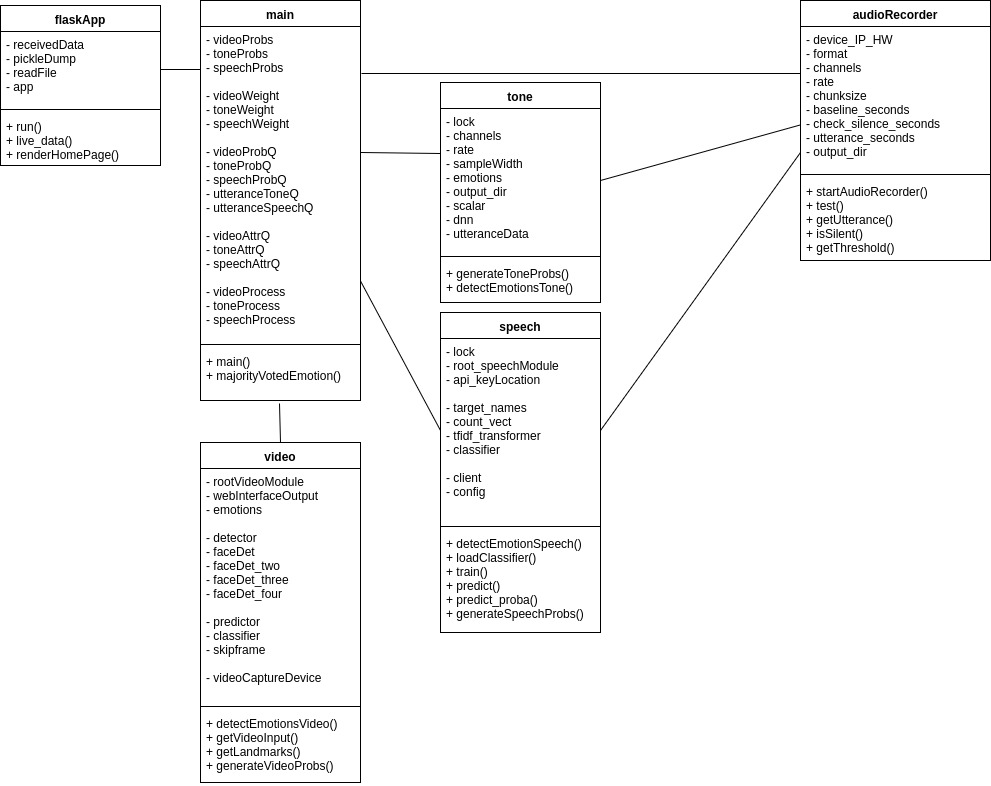
\includegraphics[width=450pt]{classDiagramProject.jpg}
		\caption{Class Diagram}
		\label{fig:class-dig}
	\end{figure}
\end{center} 

 
\subsection{Activity Diagram:}
\begin{center}
	\begin{figure}[!htbp]
		\centering
		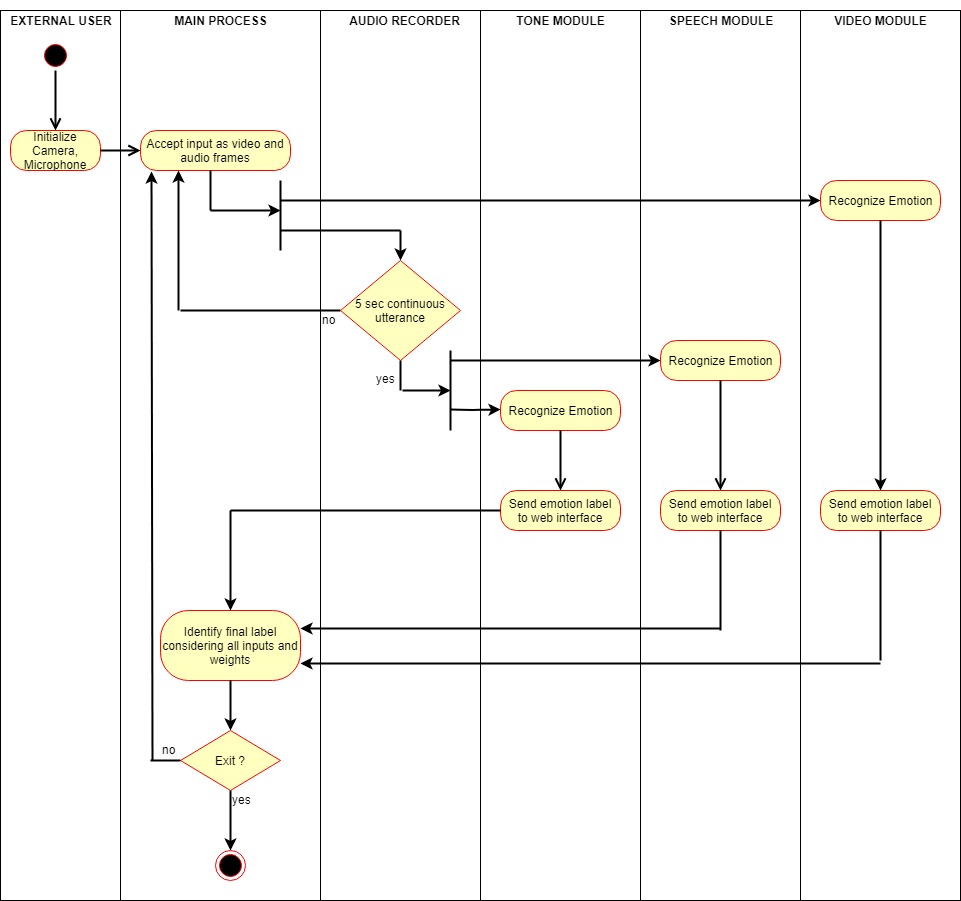
\includegraphics[width=\textwidth]{activity_proj.jpg}
		\caption{Activity Diagram}
		\label{fig:activitydiag}
	\end{figure}
\end{center}  

\subsection{State Diagram:}
\begin{center}
	\begin{figure}[!htbp]
		\centering
		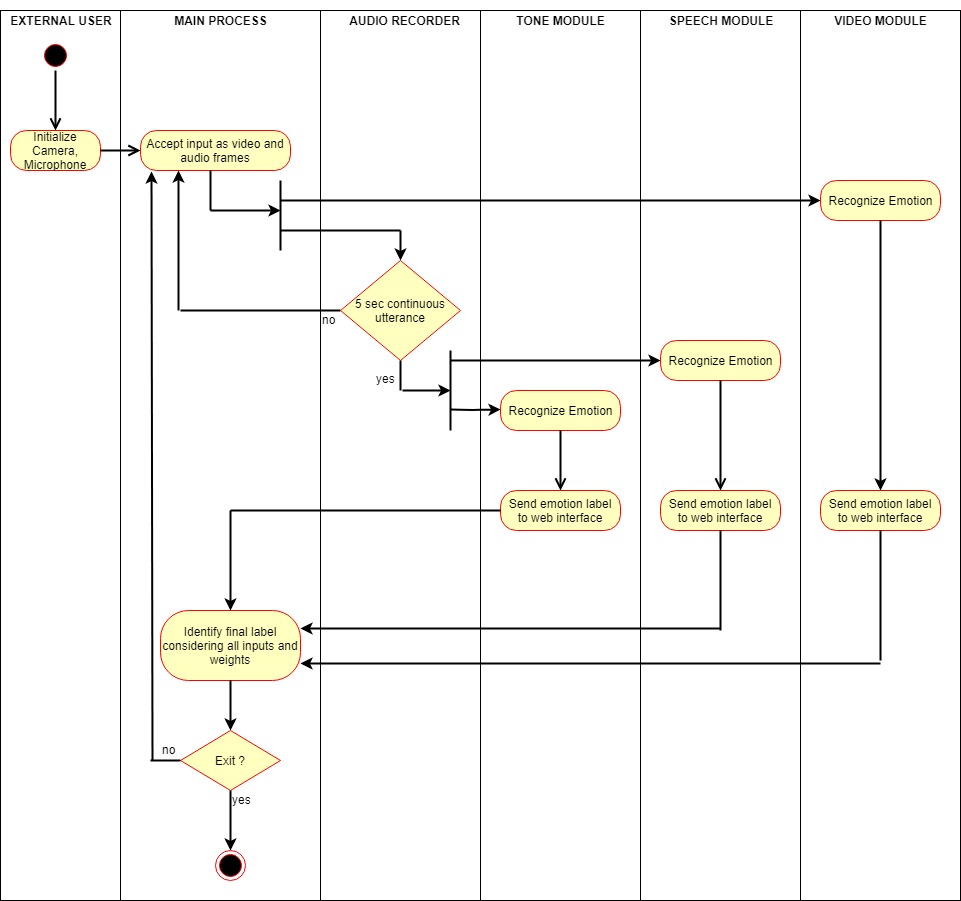
\includegraphics[width=\textwidth]{activity_proj.jpg}
		\caption{State Diagram}
		\label{fig:statediag}
	\end{figure}
\end{center}  

\subsection{Non Functional Requirements:}
\begin{itemize}
	\item The system should be near real-time.
	\item System should be able to handle multiple computations executing simultaneously and potentially iteracting with each other
	\item System should be able to store data to be communicated between processors
	\item The file system should have enough space for interprocessor communication
	\item The system will require continuous and frequent updates for the training models to improve accuracy
	\item Proper and insightful documentation is to be maintained
\end{itemize} 


\section{Architectural Design}  
 
\begin{center}
	\begin{figure}[!htbp]
		\centering
		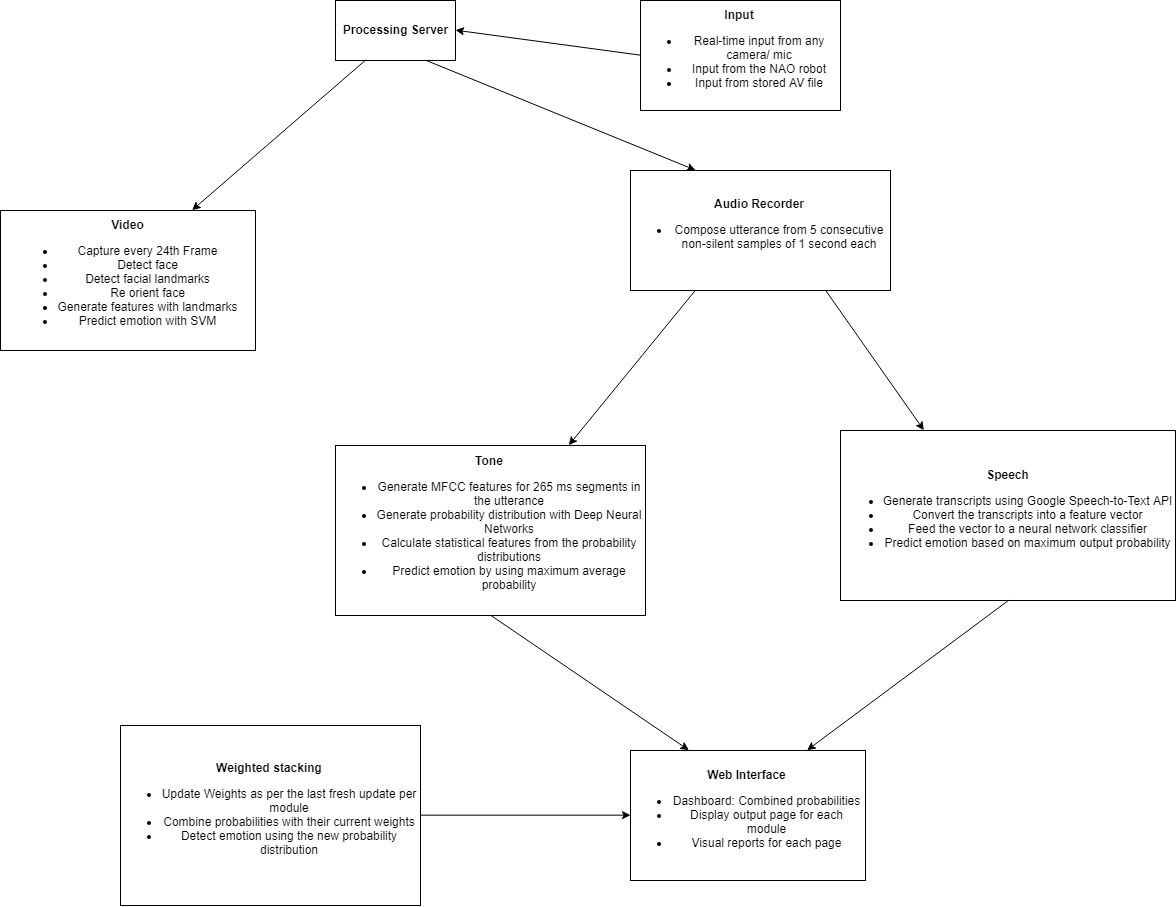
\includegraphics[width=\textwidth]{arch.jpg}
	  \caption{Architecture diagram}
	  \label{fig:arch-dig}
	\end{figure}
\end{center} 
 
\chapter{Project Implementation}
  \section{Introduction}
  
  \section{Tools and Technologies Used}
  
  \section{Methodologies/Algorithm Details}

  \subsection{Algorithm 1/Pseudo Code}
  \begin{verbatim}
  initialize videoWeight = 1
  initialize toneWeight = 1
  initialize speechWeight = 1
  
  initialize and start video subprocess
  initialize and start audioRecorder subprocess
  initialize and start tone subprocess 
  initialize and start speech subprocess
  
  Repeat till exit:
  
  If new videoProbabilities are predicted:
  		sendToGraph(videoProbs)
  		videoWeight = 1
  else:
  		decrease videoWeight by linear function
  
  If new toneProbabilities are predicted:
  		sendToGraph(toneProbs)
  		toneWeight = 1
  else:
  		decrease toneWeight by linear function
  
  If new speechProbabilities are predicted:
  		sendToGraph(speechProbs)
  		speechWeight = 1
  else:
  		decrease speechWeight by linear function
  		
  TODO: DESCRIPTION
  \end{verbatim}
 
  
  \section{Reports for classifier training process: }
	\begin{itemize}
		\item \textbf{Tone Analysis: }
			\begin{itemize}
				\item \textbf{DataSet used:} \newline
				\hspace{15mm}The Interactive Emotional Dyadic Motion Capture (IEMOCAP) database is an acted, multimodal and multispeaker database. It contains approximately 12 hours of audiovisual data, including video, speech, motion capture of face, text transcriptions. It consists of dyadic sessions where actors perform improvisations or scripted scenarios, specifically selected to elicit emotional expressions. IEMOCAP database is annotated by multiple annotators into categorical labels, such as anger, happiness, sadness, neutrality, as well as dimensional labels such as valence, activation and dominance. The detailed motion capture information, the interactive setting to elicit authentic emotions, and the size of the database make this corpus a valuable addition to the existing databases in the community for the study and modeling of multimodal and expressive human communication.
				
				
				\vspace{10mm}
				\item \textbf{TONE UTTERANCES BEFORE COMBINING:}
				Refer to figure \ref{fig:tone_utter_before}. For Tone analysis, we found that the dataset distribution was skewed.
				\begin{itemize}
				\item Anger 1103
				\item Disgust 2
				\item Excitment 1041
				\item Fear 40
				\item Frustration 1849
				\item Happiness 595
				\item Neutral 1708	
				\item Other 3
				\item Sad 1084
				\item Surprise 107
				
				\item total : 7532
			\end{itemize}	
				\vspace{10mm}
				\item \textbf{TONE UTTERANCES AFTER COMBINING:}
				Refer to figure \ref{fig:tone_utter_after}. To balance the dataset, we combined emotions with similar annotations:
				\begin{itemize}
					\item 	ang fru 2952
					\item happ exc sur 1743
					\item neutral 1708
					\item sadness fear 1124
				\end{itemize}
		
			\end{itemize}
		
		\begin{center}
			\begin{figure}[!htbp]
				\centering
				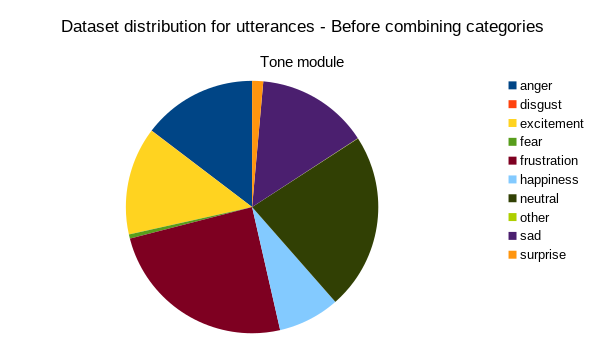
\includegraphics[width=\textwidth]{tone-utterances-before-combining.png}
				\caption{Tone Utterances before combining labels}
				\label{fig:tone_utter_before}
			\end{figure}
		\end{center}  
		\vspace{5mm}
		\begin{center}
			\begin{figure}[!htbp]
				\centering
				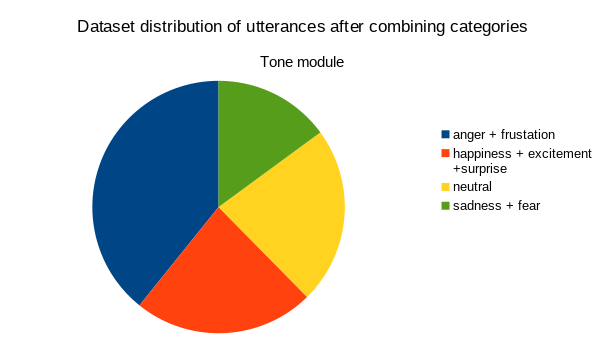
\includegraphics[width=\textwidth]{tone-utterances-after-combining.png}
				\caption{Tone Utterances after combining labels}
				\label{fig:tone_utter_after}
			\end{figure}
		\end{center}
	
		 
		\item \textbf{Training and Validation report: }
		python trainDNN.py
		Dataset loaded into dataframe...
		X and y loaded....
		Training and testing sets created...
		\(X_train\) and \(X_test\) normalized...
		Training DNN...
		Iteration 1, loss = 1.19501334 \\
		Validation score: 0.495714\\
		Iteration 2, loss = 1.02921240\\
		Validation score: 0.579298\\
		Iteration 3, loss = 0.83500359\\
		Validation score: 0.659660\\
		Iteration 4, loss = 0.63884454\\
		Validation score: 0.723208\\
		Iteration 5, loss = 0.48286869\\
		Validation score: 0.761533\\
		Iteration 6, loss = 0.37261158\\
		Validation score: 0.798439\\
		Iteration 7, loss = 0.29365010\\
		Validation score: 0.815581\\
		Iteration 8, loss = 0.23836988\\
		Validation score: 0.833706\\
		Iteration 9, loss = 0.20316889\\
		Validation score: 0.844625\\
		Iteration 10, loss = 0.17408951\\
		Validation score: 0.842660\\
		Iteration 11, loss = 0.16278715\\
		Validation score: 0.854015\\
		Iteration 12, loss = 0.14406390\\
		Validation score: 0.864825\\
		Iteration 13, loss = 0.13786938\\
		Validation score: 0.870394\\
		Iteration 14, loss = 0.13181086\\
		Validation score: 0.872304\\
		Iteration 15, loss = 0.12003902\\
		Validation score: 0.875908\\
		Iteration 16, loss = 0.11500236\\
		Validation score: 0.874707\\
		Iteration 17, loss = 0.11445793\\
		Validation score: 0.878201\\
		Iteration 18, loss = 0.10277859\\
		Validation score: 0.881858\\
		Iteration 19, loss = 0.10925041\\
		Validation score: 0.883988\\
		Iteration 20, loss = 0.09472984\\
		Validation score: 0.888246\\
		Iteration 21, loss = 0.10075731\\
		Validation score: 0.887973\\
		Iteration 22, loss = 0.09333517\\
		Validation score: 0.884370\\
		Iteration 23, loss = 0.09320555\\
		Validation score: 0.886335\\
		Validation score did not improve more than tol=0.000100 for two consecutive epochs. Stopping.\\
		DNN trained in 234.56247210502625 seconds ...\\
		TRAINING SET SCORE : 0.965337\\
		TESTING SET SCORE : 0.887380\\
		CONFUSION MATRIX for testing data : \\
		\begin{verbatim}
		[[10097   408   568   375]
		[  549 10147   369   382]
		[  447   201 10331   469]
		[  544   319   526 10059]]

		CLASSIFICATION REPORT for testing data :
		precision    recall  f1-score   support
		
		0       0.87      0.88      0.87     11448
		1       0.92      0.89      0.90     11447
		2       0.88      0.90      0.89     11448
		3       0.89      0.88      0.88     11448
		
		avg / total       0.89      0.89      0.89     45791
		\end{verbatim}
		
				\begin{center}
				\begin{figure}[!htbp]
					\centering
					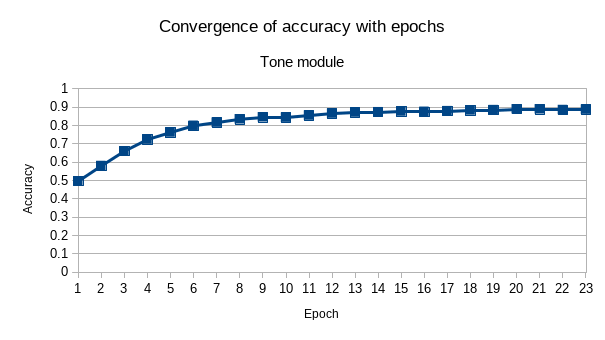
\includegraphics[width=\textwidth]{tone-convergence-dnn.png}
					\caption{Learning Curve}
					\label{fig:learning-curve}
				\end{figure}
			\end{center}

		\begin{center}
			\begin{figure}[!htbp]
				\centering
				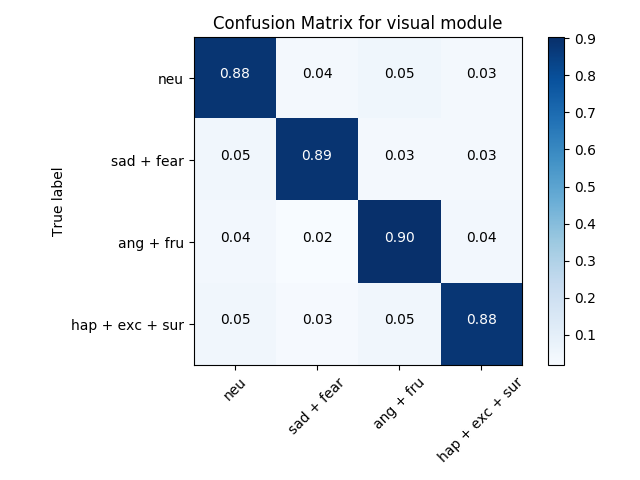
\includegraphics[width=\textwidth]{tone-confusion-matrix.png}
				\caption{Confusion Matrix}
				\label{fig:confusion_matrix}
			\end{figure}
		\end{center} 
	
		\item \textbf{Video Module: }
	\begin{itemize}
		\item \textbf{Dataset used:}\\
		\hspace{15mm}The Cohn-Kanade AU-Coded Facial Expression Database is for research in automatic facial image analysis and synthesis and for perceptual studies. Cohn-Kanade is available in two versions and a third is in preparation.
		\hspace{15mm}We have used the second version of this dataset, referred to as CK+. It includes both posed and non-posed (spontaneous) expressions and additional types of metadata. The target expression for each sequence is fully FACS coded. In addition validated emotion labels are present in the metadata. Thus, sequences may be analyzed for both action units and prototypic emotions. Additionally, CK+ provides protocols and baseline results for facial feature tracking and action unit and emotion recognition. 
		\newline
		\item \textbf{VISUAL CORPUS DISTRIBUTION:}
		We trained on 6 emotions present in the dataset with distribution as follows:\\
		Anger 45\\
		Disgust 58\\
		Happiness 69\\
		Neutral 117\\
		Sadness 28\\
		Surprise 83\\
		
		\begin{center}
			\begin{figure}[!htbp]
				\centering
				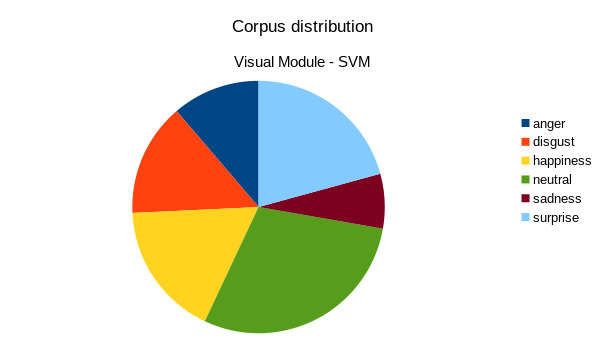
\includegraphics[width=\textwidth]{visual-corpus-distribution.png}
				\caption{Visual Corpus Distribution}
				\label{fig:visual_corpus_dist}
			\end{figure}
		\end{center}
		
		
		\item \textbf{Training and Validation Report: }\\
		Refer to figure \ref{fig:visual_learn_curv} and \ref{fig:confusion_matrix_2}
		\begin{verbatim}
		python \(classifier_for_metrics.py\)
		Making sets 0
		working on anger
		working on disgust
		working on happiness
		working on neutral
		working on sadness
		working on surprise
		training SVM linear 0
		getting accuracies 0
		linear:  0.8181818181818182
		Making sets 1
		working on anger
		working on disgust
		working on happiness
		working on neutral
		working on sadness
		working on surprise
		training SVM linear 1
		getting accuracies 1
		linear:  0.8181818181818182
		Making sets 2
		working on anger
		working on disgust
		working on happiness
		working on neutral
		working on sadness
		working on surprise
		training SVM linear 2
		getting accuracies 2
		linear:  0.7922077922077922
		Making sets 3
		working on anger
		working on disgust
		working on happiness
		working on neutral
		working on sadness
		working on surprise
		training SVM linear 3
		getting accuracies 3
		linear:  0.8701298701298701
		Making sets 4
		working on anger
		working on disgust
		working on happiness
		working on neutral
		working on sadness
		working on surprise
		training SVM linear 4
		getting accuracies 4
		linear:  0.8051948051948052
		Making sets 5
		working on anger
		working on disgust
		working on happiness
		working on neutral
		working on sadness
		working on surprise
		training SVM linear 5
		getting accuracies 5
		linear:  0.8961038961038961
		Making sets 6
		working on anger
		working on disgust
		working on happiness
		working on neutral
		working on sadness
		working on surprise
		training SVM linear 6
		getting accuracies 6
		linear:  0.7662337662337663
		Making sets 7
		working on anger
		working on disgust
		working on happiness
		working on neutral
		working on sadness
		working on surprise
		training SVM linear 7
		getting accuracies 7
		linear:  0.8701298701298701
		Making sets 8
		working on anger
		working on disgust
		working on happiness
		working on neutral
		working on sadness
		working on surprise
		training SVM linear 8
		getting accuracies 8
		linear:  0.8441558441558441
		Making sets 9
		working on anger
		working on disgust
		working on happiness
		working on neutral
		working on sadness
		working on surprise
		training SVM linear 9
		getting accuracies 9
		linear:  0.7792207792207793
		[0.8181818181818182, 0.8181818181818182, 0.7922077922077922, 0.8701298701298701, 0.8051948051948052, 0.8961038961038961, 0.7662337662337663, 0.8701298701298701, 0.8441558441558441, 0.7792207792207793]
		Mean value lin svm: 0.825974025974026
		[[ 6  2  0  1  0  0]
		[ 1 10  0  0  0  0]
		[ 0  0 13  0  0  0]
		[ 2  0  0 16  4  1]
		[ 1  0  0  1  3  0]
		[ 0  0  1  1  2 12]] 
		\end{verbatim}
		
		\begin{center}
			\begin{figure}[!htbp]
				\centering
				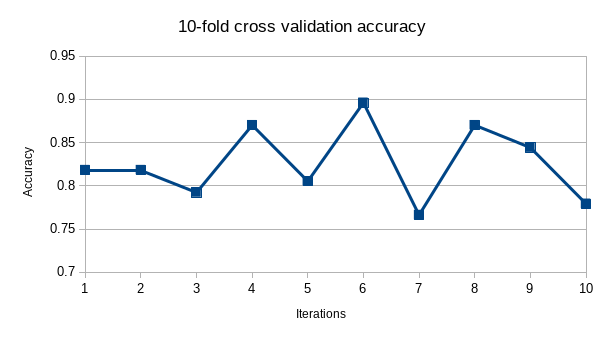
\includegraphics[width=\textwidth]{visual-kfold-svm.png}
				\caption{Learning Curve}
				\label{fig:visual_learn_curv}
			\end{figure}
		\end{center} 
		\begin{center}
			\begin{figure}[!htbp]
				\centering
				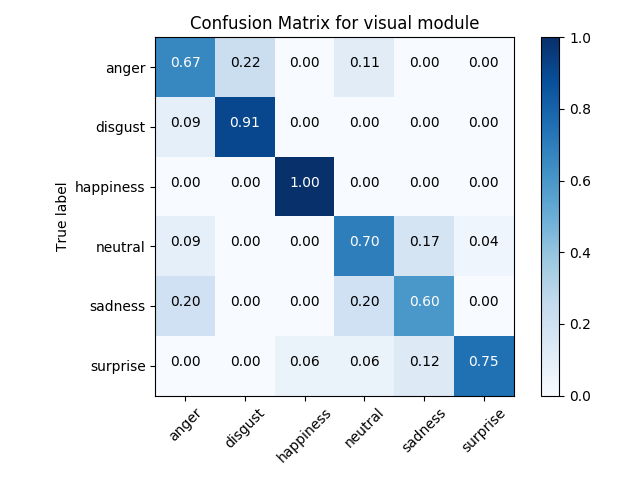
\includegraphics[width=\textwidth]{visual-confusion-matrix.png}
				\caption{Confusion Matrix}
				\label{fig:confusion_matrix_2}
			\end{figure}
		\end{center} 
		
	\end{itemize}
	
	\item \textbf{Text Analysis: }
	
	\begin{itemize}
			\item \textbf{DataSet used:} \newline
		\hspace{15mm}The Interactive Emotional Dyadic Motion Capture (IEMOCAP) database is an acted, multimodal and multispeaker database. It contains approximately 12 hours of audiovisual data, including video, speech, motion capture of face, text transcriptions. It consists of dyadic sessions where actors perform improvisations or scripted scenarios, specifically selected to elicit emotional expressions. IEMOCAP database is annotated by multiple annotators into categorical labels, such as anger, happiness, sadness, neutrality, as well as dimensional labels such as valence, activation and dominance. The detailed motion capture information, the interactive setting to elicit authentic emotions, and the size of the database make this corpus a valuable addition to the existing databases in the community for the study and modeling of multimodal and expressive human communication. For speech analysis, we use the transcripts of utterances having the same label by atleast 2 human annotaters.
			
			\vspace{5mm}
				\item \textbf{TONE UTTERANCES AFTER COMBINING:}
			Refer to figure \ref{tone-utter-after}. To balance the dataset, we combined emotions with similar annotations:
			\begin{itemize}
				\item 	ang fru 2952
				\item happ exc sur 1743
				\item neutral 1708
				\item sadness fear 1124
			\end{itemize}
		
			\begin{center}
			\begin{figure}[!htbp]
				\centering
				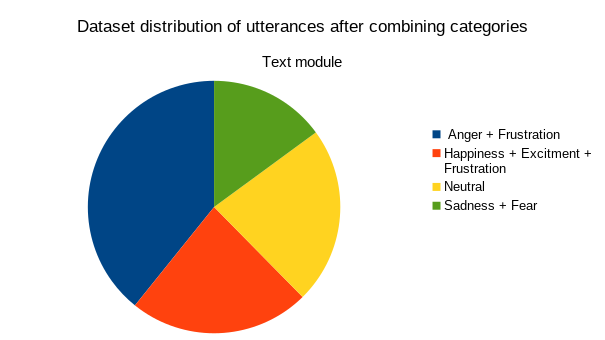
\includegraphics[width=\textwidth]{text-utterance-after-combining.png}
				\caption{Text Utterance After Combining}
				\label{fig:text-uttr-after-comb}
			\end{figure}
		\end{center} 
		
		\item \textbf{Training and Validation Report:}
		Refer to figures \ref{fig:text-convergence} and \ref{fig:text-confusion-matrix}
		\begin{verbatim}
		Iteration 1, loss = 1.36541914
		Validation score: 0.537838
		Iteration 2, loss = 1.26958823
		Validation score: 0.559459
		Iteration 3, loss = 1.13363359
		Validation score: 0.572973
		Iteration 4, loss = 0.96703096
		Validation score: 0.602703
		Iteration 5, loss = 0.81985095
		Validation score: 0.629730
		Iteration 6, loss = 0.70764039
		Validation score: 0.632432
		Iteration 7, loss = 0.62687694
		Validation score: 0.637838
		Iteration 8, loss = 0.56570615
		Validation score: 0.645946
		Iteration 9, loss = 0.51973502
		Validation score: 0.654054
		Iteration 10, loss = 0.48257364
		Validation score: 0.651351
		Iteration 11, loss = 0.45411557
		Validation score: 0.651351
		Iteration 12, loss = 0.42749150
		Validation score: 0.643243
		Validation score did not improve more than tol=0.000100 for two consecutive epochs. Stopping.
		[[102  31  42  25]
		[ 23 137  25  15]
		[ 29  24 132  15]
		[ 25  23  17 135]]
	\end{verbatim}
		\begin{center}
			\begin{figure}[!htbp]
				\centering
				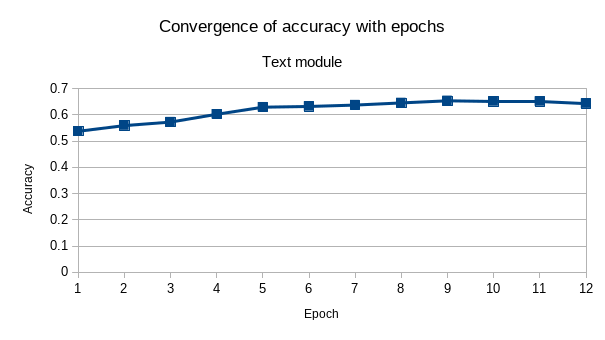
\includegraphics[width=\textwidth]{text-convergence.png}
				\caption{Text Learning Curve}
				\label{fig:text-convergence}
			\end{figure}
		\end{center} 
		
		
		\begin{center}
			\begin{figure}[!htbp]
				\centering
				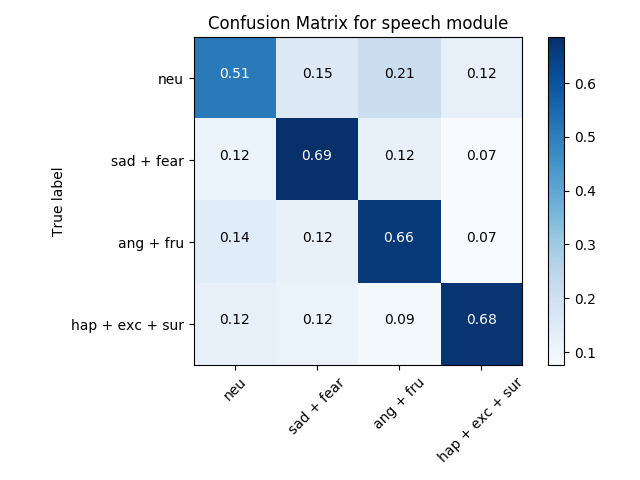
\includegraphics[width=\textwidth]{text-confusion-matrix.png}
				\caption{Text Confusion Matrix}
				\label{fig:text-confusion-matrix}
			\end{figure}
		\end{center} 
		
		
	\end{itemize}
\end{itemize}


  
  
\chapter{Software Testing}
 \section{Type of Testing Used}
   Unit,Integration,system etc.
   \section{Test Cases and Test Results}
   for each type of testing done.    
   
\chapter{Results}
\section{Screen shots}
Outputs / Snap shots of the results
\section{Outputs}

    Outputs / Snap shots of the results
\chapter{Deployment and Maintenance}
    \section{INSTALLATION:}
    \begin{itemize}
    
    
    \item Ensure you have Python 3.6 installed on a 64-bit Linux distro.
    
    \item You will need a Google cloud API key for converting speech to 
    text. Get one from : \begin{verbatim}https://cloud.google.com/docs/authentication/api-keys#creating_an_api_key \end{verbatim}
    
     \item A brief description about the project structure:
     \begin{itemize}
     	 \item envDoc : Contains all configuration files and dependencies.
     	 \item realTimeModules : Contains implementations of each individual module and also a main process to spawn subprocesses for each module.
     	 \item static : Contains static code for Flask webapp (mostly JavaScript scripts for real time rendering on webpage). 
     	 \item templates: Contains HTML webpages for client to view.
     	 \item flask-live-chart.py : The Flask webapp.
     	 
     	 \item realTimeModules/config.json : Config file to set configurable parameters. See the file comments for all the parameters which can be configured.
     \end{itemize}
   
    \textbf{Project Structure:}
    \begin{verbatim}
    EmoRecWebInterface 
    ├── envDoc 
    │   ├── env-conda-spec-file.txt 
    │   └── env-pip-packages.txt 
    ├── flask-live-chart.py 
    ├── picklesForInterface 
    │   └── pickleFile 
    ├── README.md 
    ├── realTimeModules 
    │   ├── audioRecorder 
    │   │   ├── alsa_error.py 
    │   │   ├── audioRecorder.py 
    │   │   ├── channel_index.py 
    │   │   ├── __init__.py 
    │   │   ├── __pycache__ 
    │   │   │   ├── alsa_error.cpython-35.pyc 
    │   │   │   ├── audioRecorder.cpython-35.pyc 
    │   │   │   ├── channel_index.cpython-35.pyc 
    │   │   │   └── __init__.cpython-35.pyc 
    │   │   └── test 
    │   ├── main.py 
    │   ├── speech 
    │   │   ├── api_key.json 
    │   │   ├── __init__.py 
    │   │   ├── __pycache__ 
    │   │   │   ├── __init__.cpython-35.pyc 
    │   │   │   └── speech.cpython-35.pyc 
    │   │   ├── savefile 
    │   │   ├── speech.py 
    │   │   └── transcriptions.tsv 
    │   ├── tone 
    │   │   ├── dnnParameters.sav 
    │   │   ├── energy.py 
    │   │   ├── featureExtraction.py 
    │   │   ├── __init__.py 
    │   │   ├── __pycache__ 
    │   │   │   ├── energy.cpython-35.pyc 
    │   │   │   ├── featureExtraction.cpython-35.pyc 
    │   │   │   ├── __init__.cpython-35.pyc 
    │   │   │   └── tone.cpython-35.pyc 
    │   │   ├── scalerParameters.sav 
    │   │   ├── test 
    │   │   └── tone.py 
    │   └── video 
    │       ├── EmoRecogFacial.pkl 
    │       ├── haarcascade_frontalface_alt2.xml 
    │       ├── haarcascade_frontalface_alt_tree.xml 
    │       ├── haarcascade_frontalface_alt.xml 
    │       ├── haarcascade_frontalface_default.xml 
    │       ├── __init__.py 
    │       ├── __pycache__ 
    │       │   ├── __init__.cpython-35.pyc 
    │       │   └── video.cpython-35.pyc 
    │       ├── shape_predictor_68_face_landmarks.dat 
    │       ├── test 
    │       │   └── videoplayback.mp4 
    │       └── video.py 
    ├── static 
    │   ├── js 
    │   │   ├── dashboard.js 
    │   │   └── videoScript.js 
    │   └── video.png 
    ├── templates 
    │   ├── index.html 
    │   └── live-data.html 
    └── testVideos 
    ├── audiotionExcitementFrustrationFear.mp4 
    ├── audiotionSpanish.mp4 
    ├── auditionExcited.mp4 
    ├── auditionHappy.mp4
    
    \end{verbatim}
    
    \vspace{10mm}
    \textbf{Install dependencies:}
    \begin{itemize}
    	
    
    \item statsmodels 8.0  :\\
    Python module that provides classes and functions for the estimation of many different statistical models, as well as for conducting statistical tests, and statistical data exploration. An extensive list of result statistics are available for each estimator. 
    \newline
    \item pip 9.0.3:\\
    To install python packages.
    \newline
    \item Flask 12.2:\\
    Flask is a micro web framework written in Python, used for hosting the web server.
    \newline
    \item scikit-learn 19.1:\\
    Machine learning library used for training and predicting. 
    \newline
    \item google-auth 1.4.1 : \\
    Used for authenticating Google API key.
    \newline
    \item google-api-core 1.1.2:\\
    Dependency for google-cloud.
    \newline
    \item google-cloud-speech 34.0:\\
    Used for convering speech to text transcripts.
    \newline
	\item matplotlib 2.0:\\
    Used for plotting and visualizing data locally on the server.
    \newline
    \item numpy 1.14.2:\\
    Used for processing data vectors.
    \newline
    \item pandas 22.0:\\
    Used for quick data analysis.
    \newline
    \item python-speech-features 6.0:\\
    Used by text module.
    \newline
    \item Optionally, you can create a virtual environment using the spec file given in /envDoc.\\
    
	\end{itemize}
\vspace{10mm}
    \textbf{DEPLOYMENT : }
    \begin{itemize}
    	\item Clone the repository's master branch from https://github.com/EmoRecog/EmoRecWebInterface.git
    	\newline
    	\item Switch to appropriate virtual environment with dependencies installed.
    	\newline
    	\item Run realTimeModules/main.py to start all 3 subprocesses.
    	\newline
    	\item Run flask-live-chart.py to start Flask server.
    	\newline
    	\item You can now access the interface at <IP>:5000 (5000 is the default port).
    	\newline
    \end{itemize}   
    
   \end{itemize} 
 \chapter{Conclusion and future scope}
Write  summary , conclusion and future scope
 {}

\begin{appendices}

\chapter{References}
\bibliographystyle{unsrt}
\bibliography{references.bib}

% \chapter{ALGORITHMIC DESIGN}
\chapter{Laboratory assignments on Project Analysis of Algorithmic Design}
\begin{itemize}
\item To develop the problem under consideration and justify feasibilty using
concepts of knowledge canvas and IDEA Matrix.\\

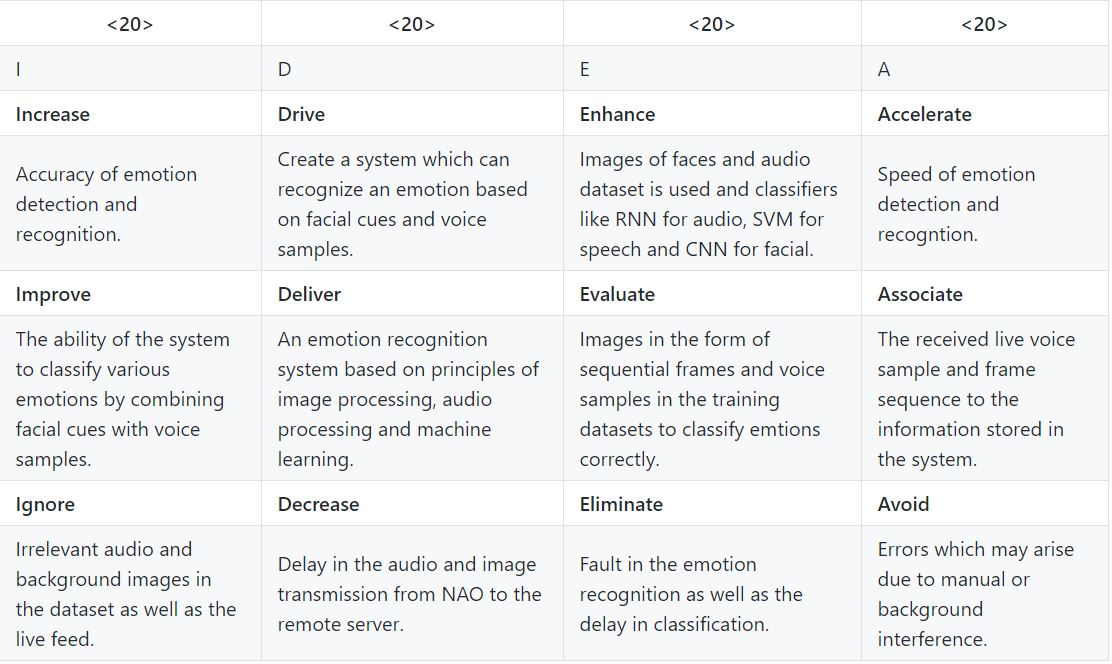
\includegraphics[width=0.7 \textheight]{idea_matrix.JPG}
\newpage
\item Project problem statement feasibility assessment using NP-Hard, NP-Complete or satisfy ability issues using modern algebra and/or relevant mathematical models.
\item input x,output y, y=f(x)
\end{itemize}

\chapter{Laboratory assignments on Project Quality and Reliability Testing of Project Design}

It should include assignments such as
\begin{itemize}
\item Use of divide and conquer strategies to exploit distributed/parallel/concurrent processing of the above to identify object, morphisms, overloading in functions (if any), and functional relations and any other dependencies (as per requirements).
             It can include Venn diagram, state diagram, function relations, i/o relations; use this to derive objects, morphism, overloading

\item Use of above to draw functional dependency graphs and relevant Software modeling methods, techniques
including UML diagrams or other necessities using appropriate tools.
\item Testing of project problem statement using generated test data (using mathematical models, GUI, Function testing principles, if any) selection and appropriate use of testing tools, testing of UML diagram's reliability. Write also test cases [Black box testing] for each identified functions. 
You can use Mathematica or equivalent open source tool for generating test data. 
\item Additional assignments by the guide. If project type as Entreprenaur, Refer \cite{ehr},\cite{mckinsey},\cite{mckinseyweb}, \cite{govwebsite}
\end{itemize}


\chapter{Project Planner}
\label{app:plan}
Using planner or alike project management tool.




\chapter{Reviewers Comments of Paper Submitted}
(At-least one technical paper must be submitted in Term-I on the project design in the
conferences/workshops in IITs, Central Universities or UoP Conferences or equivalent International Conferences Sponsored by IEEE/ACM)
\begin{enumerate}
\item Paper Title:
\item Name of the Conference/Journal where paper submitted :
\item Paper accepted/rejected : 
\item Review comments by reviewer :
\item Corrective actions if any :  

\end{enumerate}

\chapter{Plagiarism Report}
Plagiarism report
\chapter{ Term-II Project Laboratory Assignments}
\begin{enumerate}
\item Review of design and necessary corrective actions taking into consideration the feedback report of Term I assessment, and other competitions/conferences participated like IIT, Central Universities, University Conferences or equivalent centers of excellence etc.
\item Project workstation selection, installations along with setup and installation report preparations.
\item Programming of the project functions, interfaces and GUI (if any) as per 1 st Term term-work submission using corrective actions recommended in Term-I assessment of Term-work.
\item Test tool selection and testing of various test cases for the project performed and generate various testing result charts, graphs etc. including reliability testing.\\
\textbf{Additional assignments for the Entrepreneurship Project:}
\item Installations and Reliability Testing Reports at the client end.

\end{enumerate}
\chapter{Information of Project Group Members}
one page for each student .
\newpage
\begin{enumerate}
%\item Name :  \hspace{90 mm}\includegraphics[width=60pt]{photo.jpg}
\item Date of Birth :
\item Gender : 
\item Permanent Address :
\item E-Mail : 
\item Mobile/Contact No. :
\item Placement Details :
\item Paper Published : 

\end{enumerate}
\end{appendices}
\end{normalsize}
\end{document}
